\documentclass[border=10pt]{standalone}
\usepackage{tikz}
\usetikzlibrary{shapes, positioning}

\begin{document}
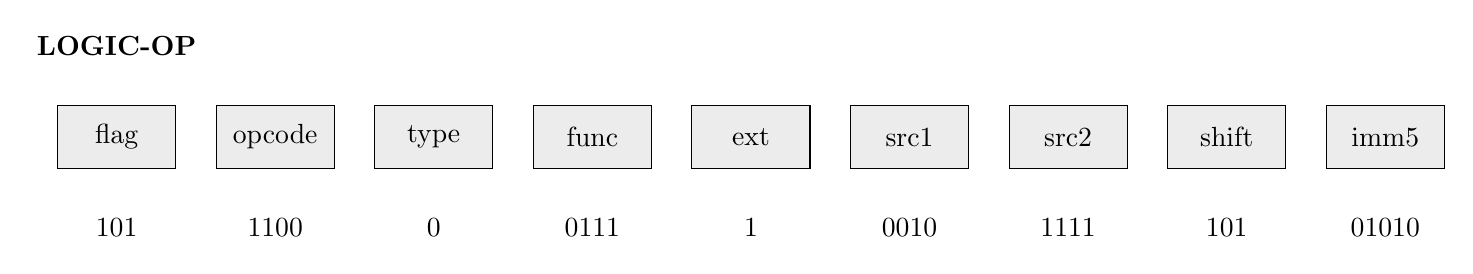
\begin{tikzpicture}[
  node distance=0.5cm,
  box/.style={rectangle, draw, fill=lightgray!30, minimum width=1.5cm, minimum height=0.8cm, align=center},
  text/.style={font=\bfseries}
]

% Boxes
\node[box] (flag) {flag};
\node[box, right=of flag] (opcode) {opcode};
\node[box, right=of opcode] (type) {type};
\node[box, right=of type] (func) {func};
\node[box, right=of func] (ext) {ext};
\node[box, right=of ext] (src1) {src1};
\node[box, right=of src1] (src2) {src2};
\node[box, right=of src2] (shift) {shift};
\node[box, right=of shift] (imm5) {imm5};

% Binary representation
\node[below=0.5cm of flag, anchor=north] {101};
\node[below=0.5cm of opcode, anchor=north] {1100};
\node[below=0.5cm of type, anchor=north] {0};
\node[below=0.5cm of func, anchor=north] {0111};
\node[below=0.5cm of ext, anchor=north] {1};
\node[below=0.5cm of src1, anchor=north] {0010};
\node[below=0.5cm of src2, anchor=north] {1111};
\node[below=0.5cm of shift, anchor=north] {101};
\node[below=0.5cm of imm5, anchor=north] {01010};

% LOGIC-OP label
\node[above=0.5cm of flag, anchor=south] {\textbf{LOGIC-OP}};

\end{tikzpicture}
\end{document}